\par \IEEEPARstart{A}{} continuaci\'on nos explayaremos sobre los detalles de la
implementaci\'on del m\'etodo propuesto. En las secciones previas hemos dado una
introducci\'on al problema, su modelo y justificaci\'on de porque el mismo sirve
y a su vez hemos expuesto un m\'etodo que nos permite hayar la soluci\'on.

\par En esta secci\'on primero hablaremos sobre una implementaci\'on del
algoritmo \ref{alg:power_method2} (p\'agina \pageref{alg:power_method2}), su
justificaci\'on y correctitud. Luego pasaremos a resolver el problema de las
estructuras de datos utilizadas para las matrices del problema (las cuales, por
representar grafos completos, presentar\'an el incoveniente al querer trabajar
con \emph{datasets} cada vez m\'as grandes).

%---------------------------------------------------------------
\subsection{Implementaci\'on del M\'etodo de la Potencia}
\par En la secci\'on previa ya se a presentado dos pseudoc\'odigos (algoritmo
\ref{alg:power_method} y \ref{alg:power_method2}) correspondiente al m\'etodo
que utilizamos durante este trabajo. El principal problema es que ambas opciones
(una siendo una versi\'on simplificada de la otra, para nuestro contexto) es que
computan $x^{(k)} \gets Mx^{(k-1)}$. Recordemos la definici\'on de nuestra
matriz $M$ entonces, de la ecuaci\'on \ref{eq:M}:

\begin{align}
    A &\in\real^{n\times n} / a_{ij} =
        \begin{cases}
            0       &\text{si $j$ no tiene links a $i$}\\
            1/n_j   &\text{si $j$ tiene links a $i$}
        \end{cases}\label{eq:A2}\\
    S &= A + \underbrace{\dfrac{1}{n}e}_{\vec{v}}a^T \quad\quad\quad
        \text{Donde: } a_i =
        \begin{cases}
            1 &\text{si el nodo $i$ es un dangling node}\\
            0 &\text{caso contrario}
        \end{cases}\label{eq:S2}\\
    M &= \alpha S + (1-\alpha)\underbrace{\overbrace{\dfrac{1}{n}e}^{\vec{v}}e^T}_E
    \label{eq:M2}
\end{align}

\par El problema, entonces, es que al computar en cada iteraci\'on $k$ del
m\'etodo de la potencia se efect\'ua la m\'ultiplicaci\'on $Mx^{k-1}$, y $M$ es
una matriz positiva (como ya se a explicado, o como se puede deducir de las
definiciones de las matrices reci\'en expuestas). Entonces tenemos que:

\begin{itemize}
    \item Cada iteraci\'on realizar\'a $2n^2-n$, es decir, $\mathcal{O}(n^2)$
        operaciones matem\'aticas. Cada fila de $M$ multiplca a
        $\vec{x}^{(k-1)}$, realizando $n$ multiplicaciones, para luego sumar
        todos sus resultados ($n-1$ sumas) y obtener una coordenada de
        $\vec{x}^{(k)}$, y esto ocurre para $n$ filas.

    \item Cuando comencemos a trabajar con muchas p\'aginas web, el tama\~no de
        la matriz crecer\'a mucho, y la complejidad espacial de la
        implementaci\'on de la matriz se volver\'a un problema de
        implementaci\'on (ni hablar cuando se trata de
        \emph{rankear}\footnote{Palabra coloquial proveniente del ingl\'es.} a
        todas las p\'aginas de internet).
\end{itemize}
\medskip

\par Kamvar et al. plantean que las aristas \emph{artificiales} introducidas en
la matriz $A$ (que representa el grafo de conectividad pesado seg\'un el grado
de salida de cada nodo) mediante $\vec{v}a^T$ y $E$ no necesitan ser
materializados en la matriz para realizar los c\'alculos (ya que de antemano
sabemos como afectan a la matriz final $M$ para cualquier operaci\'on que
hagamos con ella)~\cite[p.262]{Kamvar2003}. Por lo tanto, sugieren que el
c\'omputo de $x^{(k)} \gets Mx^{(k-1)}$ sea realizado con el siguiente
algoritmo:

\begin{algorithm}
    \KwIn{vector $\vec{x}^{(k-1)}$; matriz de conectividad pesada $A$; factor de
        navegaci\'on $\alpha$}
    \KwOut{vector $\vec{x^{(k)}}$}
    $\vec{y} \gets \alpha A \vec{x}^{(k-1)}$\;
    $w \gets ||\vec{x}^{(k-1)}||_1 - ||\vec{y}||_1$\;
    $\vec{x}^{(k)}\gets \vec{y}+w\vec{v}$\;
    \KwRet{$\vec{x}^{(k)}$}
    \caption{C\'omputo Eficiente de $x^{(k)}$\cite[p.262]{Kamvar2003}}
    \label{alg:power_method3}
\end{algorithm}

\par En un momento demostraremos que dicho algoritmo es correcto y efectivamente
est\'a computando $Mx^{(k-1)}$. Pero supongamos que asumimos esto como cierto,
¿qu\'e es lo que se gana al implementar de esta manera $Mx^{(k-1)}$?

\begin{wrapfigure}[24]{l}{0.5\textwidth}
    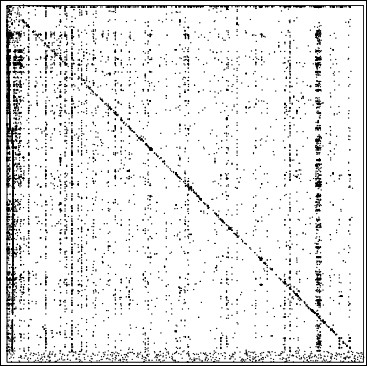
\includegraphics[width=0.48\textwidth]{example6_sparse_google_matrix.jpg}
    \caption{Ejemplo de Matriz Esparsa. Los valores no nulos est\'an indicados
    en negro~\cite[p.34]{Langville2006}}
    \label{fig:sparse_matrix}
\end{wrapfigure}

\par En primer lugar, observemos que nunca se utiliza la matriz $M$, sino que se
usa $A$. Recordemos de la definici\'on de $A$ que la misma es una matriz de
conectividad tal que $a_{ij} = \rfrac{1}{n_j}$ si hay un link de $j$ a $1$ y en
caso contrario sera nulo. Lo interesante a retener, a partir de la definici\'on
de $A$ y algo de conocimiento del dominio del problema, es que para casos muy
grandes la matriz $A$ comienza a ser cada vez m\'as esparsa. Esto ocurre porque
cada p\'agina tiene una cantidad muy acotada de links respecto de la cantidad de
p\'aginas web de internet.

\par En la figura \ref{fig:sparse_matrix} se puede observar un ejemplo real de
una matriz $A$, donde todos los valores son nulos excepto por los pixeles en
negro.

\par As\'i pues, llegamos a computar nuestro $Mx^{(k-1)}$ con una matriz
esparsa. Esto lleva a solucionarnos los 2 problemas planteados de este
c\'omputo. Por un lado las matrices esparsas pueden ser almacenadas utilizando
muy poco espacio en memoria (mediante el uso de estructuras de datos que solo
almacenan los valores no nulos m\'as alguna otra informaci\'on, las cuales
veremos un poco m\'as adelante). Por el otro, la multiplicaci\'on matriz-vector
con una matriz esparsa requiere una complejidad mucho menor que
$\mathcal{O}(n^2)$ operaciones matem\'aticas. De hecho, requiere
$\mathcal{O}(nnz(A))$, para $nnz(A)$ la cantidad de valores no nulos de $A$.
Valores estad\'isticos muestran que la cantidad promedio de links de una
p\'agina web es alrededor de 10, lo que se\~nalar\'ia que $nnz(A)=10n$ en
lugar de los $n^2$ de la matriz $M$~\cite[p.34]{Langville2006}. Entonces pasamos
de tener una complejidad $\mathcal{O}(n^2)$ a $\mathcal{O}(n)$ (por supuesto,
la implementaci\'on deber\'a permitir acceder y conocer la posici\'on de los
elementos no nulos de manera eficiente).

\par Claramente, entonces, tendr\'iamos los dos problemas planteados resueltos
en caso de ser equivalentes el c\'omputo de $x^{(k)}\gets Mx^{(k-1)}$ y el
algoritmo \ref{alg:power_method3} propuesto  Luego s\'olo quedar\'ia decidir que
estructura(s) de matrices esparsas utilizar.

%---------------------------------------------------------------
\subsection{Correctitud de C\'omputo de $\mathbf{x^{(k)}\gets Mx^{(k-1)}}$}
\begin{align}
    \intertext{Del algoritmo \ref{alg:power_method3}, reemplazando sus 3 pasos
        principales el uno en el otro, llegamos a que el $x^{(k)}$ devuelto
        ser\'a:}
    &\vec{x}^{(k)} = \alpha A \vec{x}^{(k-1)} + (||\vec{x}^{(k-1)}||_1 - ||\alpha
        A\vec{x}^{(k-1)}||_1)\vec{v}\\
    %
    \intertext{Dado que queremos demostrar que el algoritmo efectivamente
        computa $Mx^{(k-1)}$, lo que queremos demostrar es:}
    &M\vec{x}^{(k-1)} = \alpha A \vec{x}^{(k-1)} + (||\vec{x}^{(k-1)}||_1 -
    ||\alpha A\vec{x}^{(k-1)}||_1)\vec{v}\\
    %
    \intertext{Se puede observar en esto que queremos demostrar, ahora
    s\'olo tenemos $\vec{x}^{(k-1)}$, por lo tanto para facilitar la lectura nos
    referiremos al mismo como $\vec{x}$. Entonces: }
    \text{QVQ: }& M\vec{x} = \alpha A \vec{x} + (||\vec{x}||_1 - ||\alpha
    A\vec{x}||_1)\vec{v}\label{eq:qvq_dem}\\
    %
    \intertext{De las ecuaciones \ref{eq:A2}, \ref{eq:S2} y \ref{eq:M2}, podemos
    llegar a la siguiente definici\'on de $M$:}
    &\begin{aligned}
        M &= \alpha S + (1-\alpha)\vec{v}e^T\\
          &= \alpha(A+\vec{v}a^T)+(1-\alpha)\vec{v}e^T\\
          &= \alpha A+\alpha\vec{v}a^T+\vec{v}e^T-\alpha\vec{v}e^T\\
          &= \alpha A+\vec{v}(e^T-\alpha(e^T-a^T))
    \end{aligned}\\
    %
    \intertext{Luego, multiplicamos por $\vec{x}$}
    &M\vec{x} = \alpha
        A\vec{x} + \vec{v}(\underbrace{e^T\vec{x} - \alpha(e^T\vec{x} -
        a^T\vec{x})}_{\overset{?}{=} ||\vec{x}||_1 - ||\alpha
        A\vec{x}||_1})\label{eq:Mx}\\
    %
    \intertext{Analicemos en primer lugar $e^T\vec{x}$ de esta \'ultima
    ecuaci\'on. Recordemos que $\vec{x}$ era un vector est\'ocastico, entonces:}
    & e^T\vec{x} = \sum_{i=1}^{n}x_i\overarrow[=][\downarrow]{$x_i\geq 0$}
    \sum_{i=1}^{n}|x_i| = ||\vec{x}||_1\label{eq:reemp1}\\
    %
    \intertext{Por otro lado, analicemos $||A\vec{x}||_1$}
    &\begin{aligned}
        ||A\vec{x}||_1 &= \sum_{i=1}^{n} \left|\sum_{j=1}^n a_{ij}x_j\right|
            \overarrow[=][\downarrow]{$a_{ij}\geq 0$\\[-15pt]\tiny$x_j\geq 0$}
                \sum_{i=1}^{n} \sum_{j=1}^n |a_{ij}| |x_j|
            =
                \sum_{j=1}^{n}|x_j| \underbrace{\left(\sum_{i=1}^n|a_{ij}|\right)}_{
                    \underarrow[=][\uparrow]{Columna $j$ de $A$ es\\[-15pt]\tiny
                    estoc\'astica si $n_j\neq 0$\\[-15pt]\tiny
                    Ecuaci\'on \ref{eq:A2}}
                    \begin{cases}
                        0 &\text{Si $n_j = 0$}\\
                        1 &\text{Si $n_j\neq 0$}
                    \end{cases}
                }
            \overarrow[=][\downarrow]{$x_i\geq 0$}
                \sum_{\substack{j=1\\n_j\neq 0}}^n x_j\label{eq:sum1}
    \end{aligned}\\
    %
    \intertext{Y ahora analicemos el t\'ermino restante de la ecuaci\'on
    \ref{eq:Mx}:}
    &e^T\vec{x}-a^T\vec{x}
        = \left(\sum_{i=1}^{n}x_i\right)
            - \left(\sum_{\substack{i=1\\n_i=0}}^n x_i\right)
        = \sum_{\substack{i=1\\n_i\neq 0}}^n x_i\label{eq:sum2}\\
    %
    \intertext{Entonces, si observamos las ecuaciones \ref{eq:sum1} y
    \ref{eq:sum2}, llegamos a que:}
    &e^T\vec{x}-a^T\vec{x} = ||A\vec{x}||_1\label{eq:reemp2}\\
    %
    \intertext{Por \'ultimo, si tomamos las igualdades obtenidas en las
    ecuaciones \ref{eq:reemp1} y \ref{eq:reemp2} y las utilizamos en la
    ecuaci\'on \ref{eq:Mx}, llegamos a que:}
    &M\vec{x} =
        \alpha A\vec{x} + \vec{v}(||\vec{x}||_1 - \alpha||A\vec{x}||_1)
    \overarrow[\implies][\downarrow]{$\alpha\geq 0$}
    M\vec{x} =
        \alpha A\vec{x} + (||\vec{x}||_1 - ||\alpha A\vec{x}||_1)\vec{v}
\end{align}

\par Que es, justamente, lo que quer\'iamos demostrar (ecuaci\'on \ref{eq:qvq_dem}).

%---------------------------------------------------------------
\subsection{Estructuras de Datos para Matrices
Esparsas\protect\footnote{T\'ermino coloquial utilizada para referirnos a
matrices poco densas, es decir matrices con muchos valores nulos.}}
\par Como se ha mencionado, la princpal ''optimizaci\'on'' de la
implementaci\'on\footnote{y m\'as que optimizaci\'on, necesidad, ya que para
instancias grandes no nos alcanzar\'ia con 16GB de memoria RAM para
instanciar la matriz.} es la utilizaci\'on de estructuras especiales para
representar matrices esparsas. Esta elecci\'on, sin embargo, debe ser
inteligente para permitir que el algoritmo \ref{alg:power_method3} funcione con
las complejidades ya enunciadas.

\par El enunciado de este trabajo menciona 3 posibles implementaciones de
matrices esparsas (secci\'on \ref{apx:sparse_matrix}, p\'agina
\pageref{apx:sparse_matrix}), las cuales enunciamos a continuaci\'on junto con
sus caracter\'isticas pertintentes a nuestro contexto:

\smallskip
\begin{LaTeXdescription}
    \item[Dictionary of Keys (DoK)] Es una estructura buena para construir la
        matriz incrementalmente con datos de entrada desordenados, pero no es
        eficiente para iterar los valores no nulos en orden, lo cual no hace a
        esta estructura no permite realizar operaciones algebr\'aicas (como
        multiplcaci\'on matriz-vector) de manera eficiente. Suele usarse para
        construir la matriz, la que luego es transformada a un formato m\'as
        eficiente para el procesamiento de los datos\cite{wiki_dok}. Es
        tambi\'en llamada en otros \'ambitos como \textbf{Hash Table
        Storage}\cite{alglib_sparse}.

    \item[Compressed Row Storage (CRS)] Es una estructura d\'ificil de
        inicializar, pues a pesar de ser eficiente en cuanto al uso de memoria,
        los datos no pueden ser insertados en orden arbitrario\footnote{No es
        que no se pueda, pero se vuelve realmente ineficiente.}. Esto nos obliga a
        pasarle los datos en un orden espec\'ifico para poder construir dicha
        estructura. Como ventaja tiene que permite realizar operaciones
        algebr\'aicas de manera eficiente, a pesar de requerir un direccionamiento
        indirecto a los elementos para acceder a los elementos una vez dada la
        posici\'on del mismo\cite{wiki_dok}\cite{alglib_sparse}.

    \item[Compressed Column Storage (CCS)] Es una estructura id\'entica a CRS
        respecto a sus caracter\'isticas. La diferencia radica en que en lugar
        de almacenar referencias a las filas, lo hace a las columnas. En otras
        palabras, podemos decir que dada una matriz $A$, CCS es el formato CRS de
        $A^T$\cite{netlib_ccs}. Al entrar m\'as en detalles en los siguientes
        p\'arrafos sobre la estructura de CRS, esto quedar\'a m\'as claro.
\end{LaTeXdescription}
\medskip

\par Observando estas caracter\'isticas, claramente afrontamos un problema.
Necesitamos una estructura para matrices esparsas que sea apta para operaciones
algebr\'aicas (como lo son CRS y CCS), pero en principio no podemos asegurar que
la informaci\'on de las instancias de entrada vengan manteniendo alg\'un orden
espec\'ifico, con lo cual la construcci\'on de dicha estructura no es viable.
Podr\'iamos usar DoK para construir sin problemas dicha instancia, pero esta
estructura no es apta para las operaciones que luego necesitaremos realizar con
ella.

\par La decisi\'on entonces fue entonces la mencionada en casi todas las
referencias: utilizamos un DoK para la instanciaci\'on de los datos, para luego
transformar dicha estructura en un formato m\'as adecuado para las operaciones
algebr\'aicas. Nuestra elecci\'on en este caso fue CRS, ya que interpretamos que
la implementaci\'on de la operaci\'on multiplicaci\'on matriz-vector era m\'as
f\'acil con \'esta que con CCS (como explicaremos dentro de unas secciones).

\par A continuaci\'on, pasamos a explicar los detalles de las estructuras
elegidas y nuestra implementaci\'on de ellas.

%---------------------------------------------------------------
\subsubsection{Dictionary of Keys (DoK)}
\par Los art\'iculos investigados al respecto describen al DoK como una tabla de
\emph{hash}, la cual almacena los datos de entrada en tiempo constante (si
asumimos que generar el hash es de tiempo constante, lo que suele ocurrir) pero
de manera desordenada. Es decir, la estructura termina siendo un diccionario
implementado sobre una tabla de hash, lo que nos da tiempo de inserci\'on,
acceso y modificaci\'on a los datos en tiempo constante.

\par En contrapartida, recorrer los elementos almacenados en orden (tanto por
clave como por valor) no es una opci\'on soportada. Ni tampoco saber, por
ejemplo, para una fila dada que elementos no nulos se tienen almacenados de la
misma (ni en que columna). Esto \'ultimo es lo que dificulta enormemente las
operaciones algebr\'aicas sobre esta estructura (consultar si hay un valor no
nulo almacenado en una posici\'on tiene costo constante, pero al multiplcar se
requiere consultar columna por columna para una fila dada, obteniendo un costo
final $\mathcal{O}(n)$ que no es mejor que lo que provee una matriz almacenada
como vector de vectores\footnote{Aunque se obtuvo una mejora en cuanto a la
complejidad espacial.}).

\par La utilidad de esta estructura, al elegirla, es la de poder realizar la
inserci\'on de datos de manera desordenada (u inserci\'on en posiciones
arbitrarias), para luego poder recorrer estos datos en forma ordenada, que es lo
que necesitamos para poder pasar a una representaci\'on CRS. Pero esto \'ultimo
no parece ser una opci\'on de una implementaci\'on cl\'asica de DoK. Llegados a
este punto, contemplamos las siguientes opciones:

\begin{itemize}
    \item Una soluci\'on ser\'ia recorrer los elementos desordenados, utilizar
        un vector temporal para ordenarlos (donde cada elemento es una terna
        $<fila,columna,valor>$) y luego utilizar los datos ordenados para
        construir un CRS.

    \item Una alternativa ser\'ia realizar diccionario basado en un
        \emph{AVL}\cite{wiki_avl} en lugar de una tabla de hash. Esto har\'ia que
        los datos est\'en ordenados internamente (por el par $<fila,columna>$),
        aunque pagar\'iamos el costo de insertar los datos de manera ordenada
        (costo que en la soluci\'on previa, pagar\'iamos al ordenar el vector
        temporal).
\end{itemize}
\smallskip

\par La segunda opci\'on planteada no es, estrictamente hablando, un DoK; ya que
si bien tenemos un diccionario que nos asocia una llave o \emph{key} con un
valor, el mismo no tiene un costo constante para inserci\'on y acceso a los
datos. Ser\'ia un DoK si solo observamos la abstracci\'on de los datos, y el
hecho de que la inserci\'on de datos desordenados (como su acceso) puede ser
realizado sin mayores problemas\footnote{Ya que la abstracci\'on de un
diccionario implementado sobre AVL ya est\'a realizada\cite{stl_map}.}.

\par Dado el uso que le daremos a esta estructura, observamos que el costo de la
primer soluci\'on es $\mathcal{O}(nnz$ $log(nnz))$ para $nnz$ la cantidad total de
valores no nulos\footnote{$\mathcal{O}(nnz)$ inserciones, $\mathcal{O}(nnz$
$log(nnz))$ para ordenar el vector y $\mathcal{O}(nnz)$ para recorrerlo.}. En la
alternativa, tendremos un costo de $\mathcal{O}(nnz$ $log(nnz))$\footnote{Crear la
matriz tend\'a costo $\sum_{i=1}^{nnz} \mathcal{O}(log(i)) = \mathcal{O}(nnz$
$log(nnz))$, y luego recorrerla en orden ser\'a $\mathcal{O}(nnz)$.}, es decir,
el costo asint\'otico en cuanto accesos/escrituras a memoria es el mismo.

\par As\'i pues decidimos ir por la segunda alternativa, por el simple hecho de
que cualquiera de las dos implementaciones se basar\'ian en la \emph{standard
library} de \emph{C++} (\emph{unordered\_map}\cite{stl_unordered_map} y
\emph{map}\cite{stl_map}), pero usando \emph{map} nos evitamos tener que crear
un vector y ordenarlo para luego construir la matriz CRS.

\par Resumiendo, nuestra implementaci\'on de (pseudo)DoK no es otra cosa que un
$diccionario< enteros,diccionario<enteros,valor>>$, donde ambos diccionarios
est\'an implementados utilizando el contenedor \emph{Map} de la \emph{stl} de
\emph{C++}, el cual utiliza como estructura interna un \'arbol AVL y nos
garantiza las complejidades enunciadas\cite{stl_map}. Los detalles m\'as
espec\'ificos sobre esta implementaci\'on se pueden encontrar en el ap\'endice
\ref{sec:codigo_relevante}.

%---------------------------------------------------------------
\subsubsection{Compressed Row Storage (CRS)}
\par Como ya hemos expresado, la implementaci\'on CRS tiene como
caracter\'isticas almacenar la informaci\'on de la matriz esparsa de forma
eficiente (sino no tendr\'ia mucho sentido) y permite implementar funciones
aritm\'eticas de manera igualmente eficiente.

\par La estructura de datos en si misma consta de 3 vectores: uno para los
valores no nulos de la matriz (llamaremos a este vector $val$) en orden de
aparici\'on de los mismos al recorrer la matriz de izquierda a derecha y de
arriba hacia abajo, otro vector ($col\_ind$) que almacena los \'indices de las
columnas de los elementos de $val$ (es decir, si $val[k] = m_{ij}$, entonces
$col\_ind[k] = j$) y por \'ultimo $row\_ptr$ que almacena los \'indices sobre
$val$ que representan el primer valor no nulo de una fila (es decir, si $val[k]
= m_{ij}$, entonces $row\_ptr[i]\leq k < row\_ptr[i+1]$). Por convenci\'on, se
define a $row\_ptr[n+1] = nnz+1$\cite{netlib_crs}.

\par Como se puede observar, finalmente se almacenan $2nnz+n+1$ valores entre
los 3 vectores, en lugar de almacenar $n^2$ si se hubiera usado la estructura
intuitiva de vector de vectores.

\par Presentamos un ejemplo a continuaci\'on, para ilustrar la idea.
Consideremos la siguiente matriz $A\in\real^{6\times 6}$\cite{netlib_crs}:

\begin{equation*}
    A = \begin{bmatrix*}[r]
        10 &0 &0 &0 &-2 &0\\[-0.65em]
         3 &9 &0 &0 &0  &3\\[-0.65em]
         0 &7 &8 &7 &0  &0\\[-0.65em]
         3 &0 &8 &7 &5  &0\\[-0.65em]
         0 &8 &0 &9 &9  &13\\[-0.65em]
         0 &4 &0 &0 &2  &-1
    \end{bmatrix*}
\end{equation*}

\par Y los vectores de la implementaci\'on CRS de esta matriz ser\'ian:

\begin{table}[!h]
    \begin{tabular}{|r|c|c|c|c|c|c|c|c|c|c|c|c|c|}
        \hline
        \textbf{val}&10&-2&3&9&3&7&8&7&3\dots 9&13&4&2&-1\\
        \hline
        \textbf{col\_ind}&1&5&1&2&6&2&3&4&1\dots 5&6&2&5&6\\
        \hline
    \end{tabular}
    \begin{tabular}{|r|c|c|c|c|c|c|c|}
        \hline
        \textbf{row\_ptr}&1&3&6&9&13&17&20\\
        \hline
    \end{tabular}
\end{table}
\medskip

\par Observando esto, queda claro el porque es complicado hacer una inserci\'on
arbitrar\'ia de elementos. Supongamos en el ejemplo que deseamos agregar un
nuevo dato no nulo $x$ en $a_{2,3}$. En primer lugar deber\'iamos incrementar el
tama\~no de $val$ en uno, para luego insertar $x$ en $val[5]$. Antes de hacer
esto, debemos mover todos los valores a partir de $val[5]$ una posici\'on dentro
de $val$, es decir $val[i]\gets val[i-1]$ para $i=5..nnz$\footnote{Asumimos que
$nnz$ incluye al nuevo valor $x$.}. Lo mismo habr\'a que hacer en $col\_ind$
para poder insertar la columna de $x$ (3) en $col\_ind[5]$. Ahora todos
\'indices de $row\_ptr$ se encuentran desactualizados, con lo cual debemos
incrementar en uno todos los \'indices a partir de la posici\'on 3, pues las
posiciones a las que hac\'ian referencia en $val$ fueron ''corridas'' una
posici\'on por el agregado de $x$.  Por \'ultimo, debemos actualizar el \'ultimo
valor almacenado en $row\_ptr$, ya que $nnz$ ha sido incrementado por la
inserci\'on de $x$.

\par En este ejemplo, con esto bastar\'ia, pero si el nuevo elemento insertado
se hubiera convertido en el nuevo primer elemento de la fila $2$, deber\'iamos a
su vez actualizar el \'indice de $val$ que nos indica el primer valor no nulo de
la fila $2$: $row\_ptr[2] \gets 5$. Todo este proceso tiene un costo total de
$\mathcal{O}(2nnz+n)$, es decir, lineal en $max(nnz,n)$. Si comparamos este
costo contra el costo de inserci\'on de un simple vector de vectores
($\mathcal{O}(1)$), o contra nuestro DoK ($\mathcal{O}(log(nnz))$), o incluso el
DoK cl\'asico ($\mathcal{O}(1)$), veremos que claramente no es eficiente esta
estructura para insertar nuevos valores. A\'un as\'i, es trivial ver que si los
valores vienen ordenados (siguiendo el orden de izquierda a derecha y de arriba
hacia abajo), la generaci\'on de estos vectores costar\'a simplemente
$\mathcal{O}(nnz)$, pues a medida que vamos iterando los valores ordenados,
debemos simplemente ir agregando elementos al final de cada uno de los vectores
(en el caso de $row\_ptr$, deberemos agregar un nuevo \'indice cuando un nuevo
valor pertenece a una fila distinta que su valor anterior).

\par Cabe aclarar que este ejemplo no contempla la posibilidad de que haya una
fila sin valores no nulos. Dado este caso, en nuestra implementaci\'on,
decidimos colocar en la posici\'on correspondiente de $row\_ptr$ un valor
interpretable como $\infty$. En nuestro caso, ese valor es el valor m\'aximo del
tipo de datos del vector (\emph{unsigned int})\cite{stl_limits}.

\par El \'ultimo aspecto que nos queda por analizar es por qu\'e esta
representaci\'on de una matriz esparsa nos sirve para realizar operaciones
aritm\'eticas (por lo menos la multiplicaci\'on matriz-vector) de manera
eficiente. Como ya hemos mencionado, si no usaramos una estructura que pueda
saber en todo momento donde est\'an los valores no nulos, al realizar la
multiplicaci\'on de cada fila por el vector nos veremos obligados a realizar
$2n-1$ operaciones matem\'aticas (las $n$ multiplicaciones y las $n-1$
adiciones), de las cuales muchas ser\'an multiplicar por $0$\footnote{Cosa que
incluso nos podr\'ia llevar a tener errores num\'ericos.} y siendo estas
operaciones innecesarias\footnote{Se podr\'ia verificar que el valor de la
matriz sea no nulo antes de efectuar la operaci\'on, pero dicha verificaci\'on
no es m\'as eficiente que realizar la multiplicaci\'on.}. Ahora bien, al
utilizar la estructura de CRS, podemos iterar por los valores no nulos de una
fila dada, y en cada caso saber exactamente cual es el \'indice del vector con
el cual deben multiplicarse: el \'indice de la columna del elemento no nulo.
As\'i pues, en cada multiplicaci\'on de vectores (fila de la matriz por vector),
estaremos realizando la cantidad justa y necesaria de operaciones matem\'aticas,
lo cual claramente hace m\'as eficente a nuestro algoritmo del m\'etodo de la
potencia, el cual depende de realizar la operaci\'on $Mx^{(k-1)}$ en cada $k$
iteraci\'on (algoritmo \ref{alg:power_method3}, p\'agina
\pageref{alg:power_method3}).

\par As\'i hemos introducido como es la estructura CRS y porque la misma sirve a
los prop\'ositos del actual trabajo: sus ventaja espaciales para almacenar
matrices esparsas y para las operaciones aritm\'eticas, sumados a su bajo costo
de inicializaci\'on si los valores no nulos de la matriz puede ser recibidos en
orden, cosa que conseguimos mediante el uso de una representaci\'on auxiliar de
la matriz: DoK.

%---------------------------------------------------------------
\subsubsection{Compressed Row Storage (CCS)}
\par Aprovechando, mencionamos que la implementaci\'on de CCS sigue exactamente
la misma idea que CRS, salvo que invierte la idea de tener \'indices a columnas
y conocer las posiciones de $val$ inician una fila por tener \'indices a filas y
conocer las posiciones de $val$ que inician una columna. En la matriz $A$ del
ejemplo anterior tendr\'iamos los siguientes vectores\cite{netlib_ccs}:

\begin{table}[!h]
    \begin{tabular}{|r|c|c|c|c|c|c|c|c|c|c|c|c|c|}
        \hline
        \textbf{val}&10&-2&3&9&3&7&8&7&3\dots 9&13&4&2&-1\\
        \hline
        \textbf{row\_ind}&1&2&4&2&3&5&6&3&4\dots 5&6&2&5&6\\
        \hline
    \end{tabular}
    \begin{tabular}{|r|c|c|c|c|c|c|c|}
        \hline
        \textbf{col\_ptr}&1&4&8&10&13&17&20\\
        \hline
    \end{tabular}
\end{table}

\par En el contexto de este trabajo optamos por utilizar la representaci\'on CRS
en lugar de \'esta, ya que a la hora de realizar la operaci\'on aritm\'etica de
mayor peso para el m\'etodo de la potencia era m\'as importante poder iterar los
valores no nulos de una fila m\'as que los de una columna (ya que debemos hacer
el producto interno de cada fila con un vector). Claramente esto no es un
obst\'aculo insalvable dentro de esta estr\'uctura (basta con transponer la
matriz y hacer los productos internos columna a columna), pero realizar esto nos
pareci\'o innecesario y poco intuitivo, m\'as a\'un teniendo que implementar
cualquier representaci\'on desde cero y pudiendo elegir CRS.

%---------------------------------------------------------------
